\lfoot{William Matthews}
\section{Power Control and Grid Balancing}




\begin{figure}[H]
\centering
        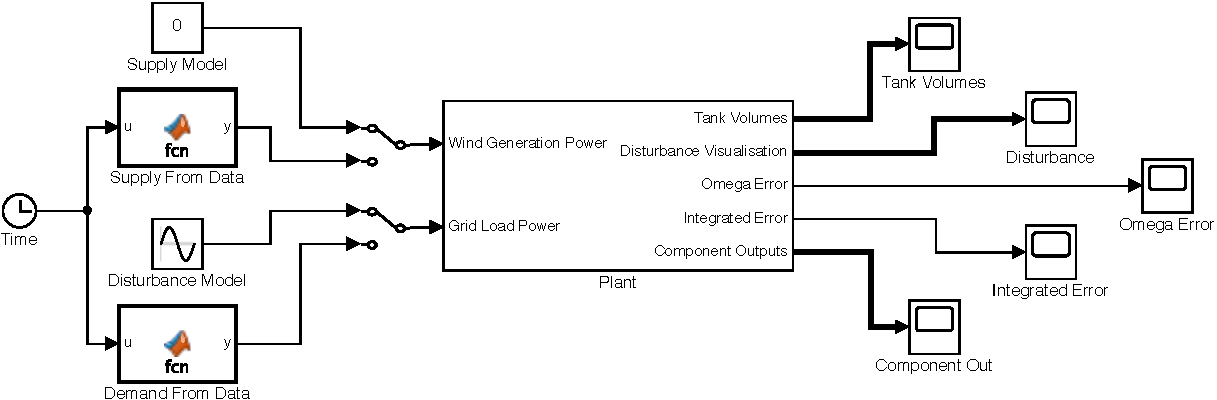
\includegraphics[scale=0.7]{images/plant/global.pdf}
        \caption{Plant in Testing Environment}
        \label{fig:global}
\end{figure}
\begin{figure}[H]
\centering
        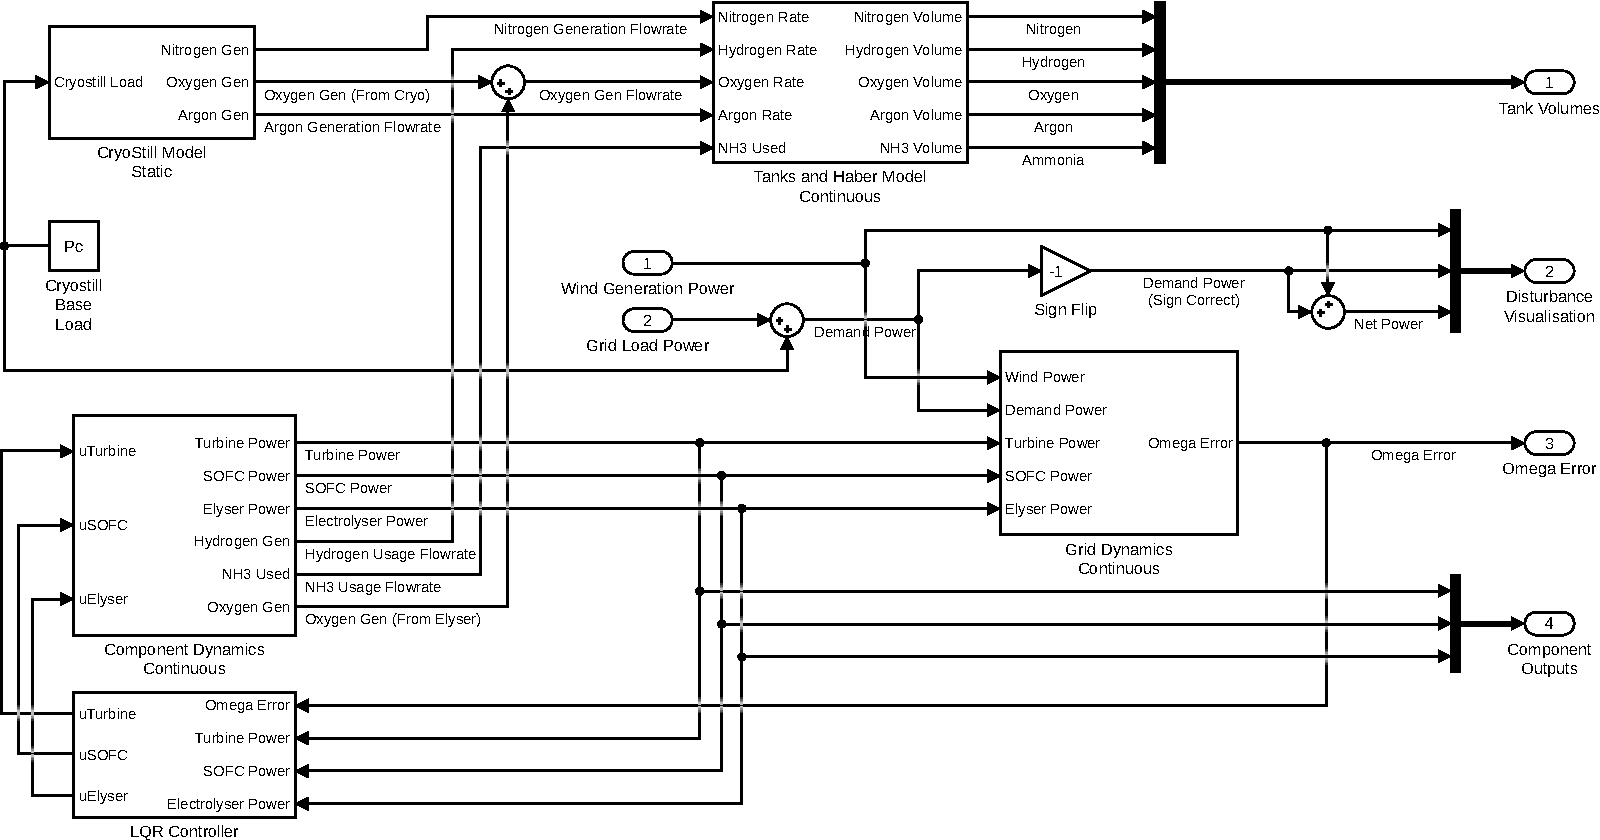
\includegraphics[scale=0.6]{images/plant2/plant.pdf}
    \caption{Plant with Controller Implemented}
        \label{fig:plant}
\end{figure}
\begin{figure}[H]
\centering
        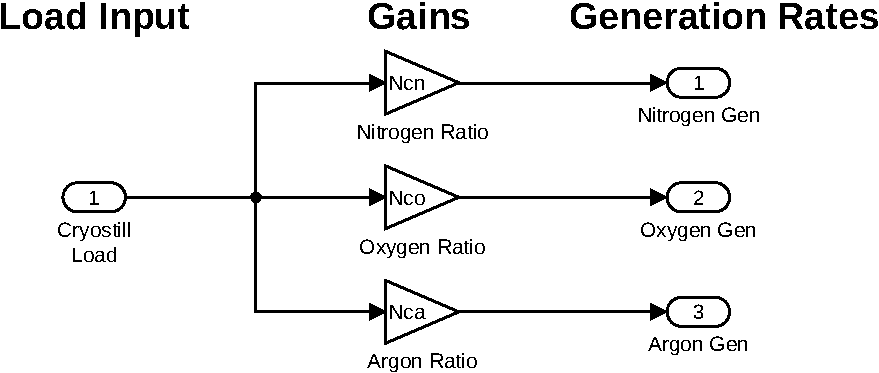
\includegraphics[scale=0.7]{images/plant2/cryo.pdf}
    \caption{Steady State Cryogenic Still Model}
        \label{fig:cryo}
\end{figure}
\begin{figure}[p]
\centering
        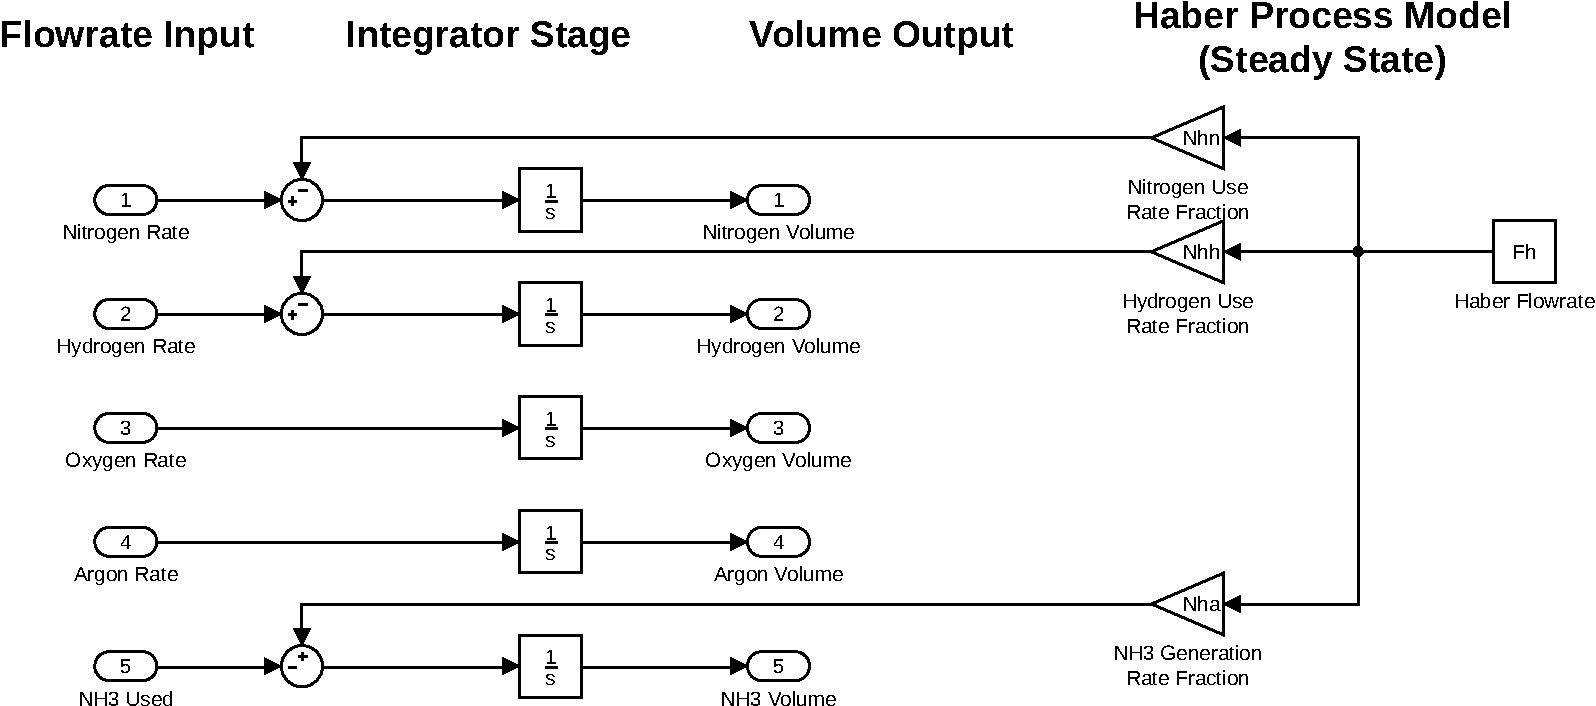
\includegraphics[scale=0.65]{images/plant2/tank.pdf}
    \caption{Tank and Steady State Haber Column Model}
        \label{fig:tank}
\end{figure}
\begin{figure}[p]
\centering
        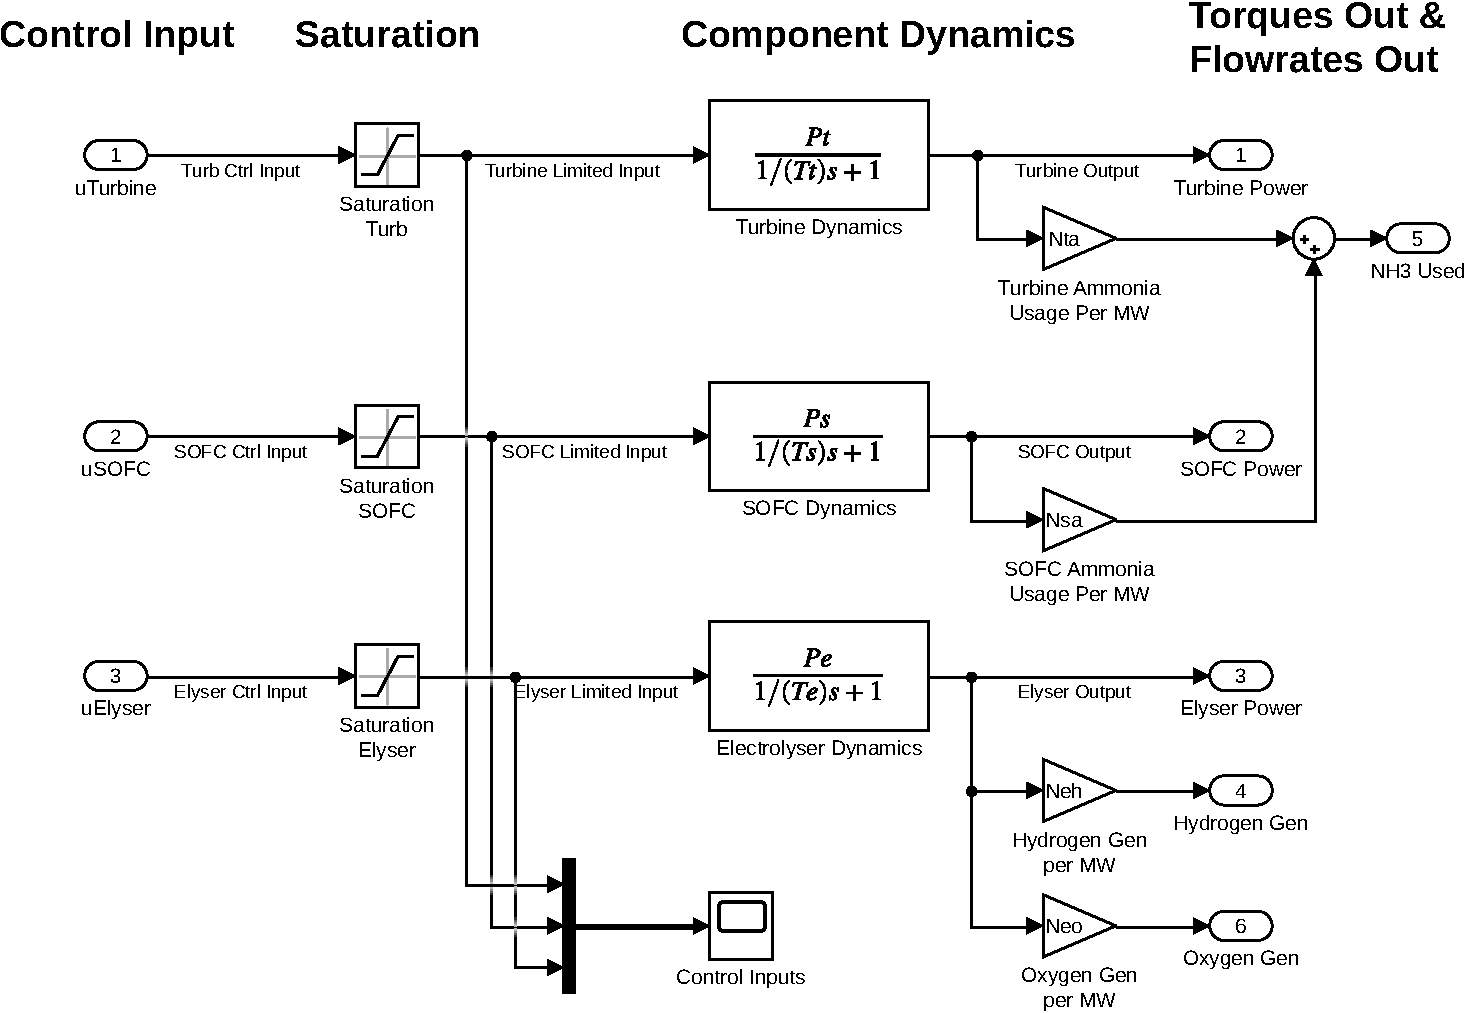
\includegraphics[scale=0.7]{images/plant2/comp.pdf}
    \caption{Component Dynamics (First Order Linear) with Saturation on Inputs}
        \label{fig:comp}
\end{figure}
\begin{figure}[p]
\centering
        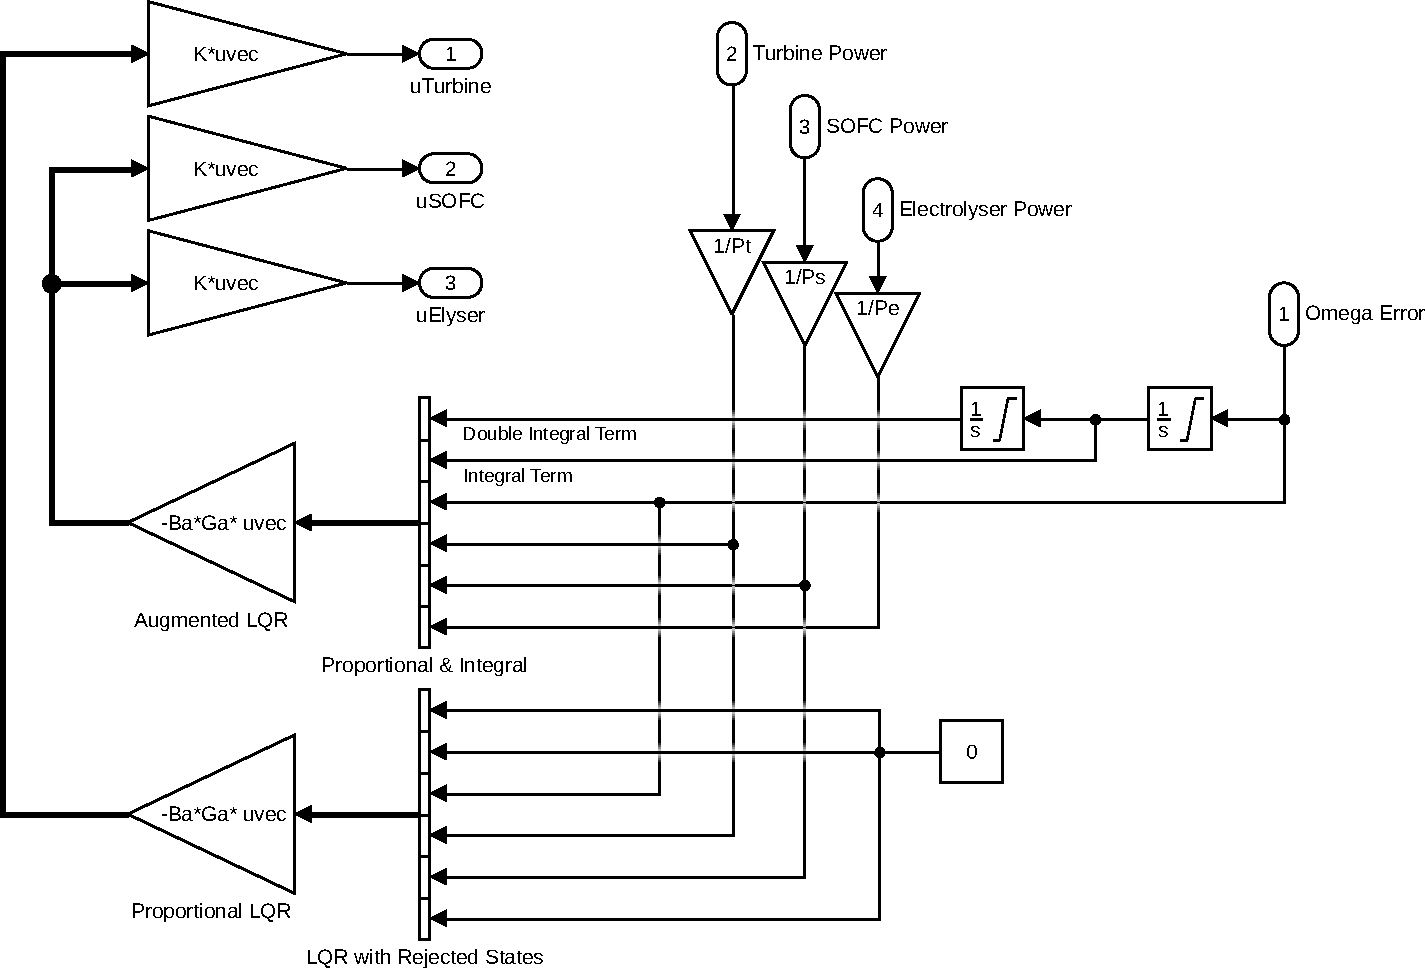
\includegraphics[scale=0.7]{images/plant2/ctrl.pdf}
    \caption{Controller Structure (LQR with Augmented State shown in Diagram)}
        \label{fig:ctrl}
\end{figure}
\begin{figure}[p]
\centering
        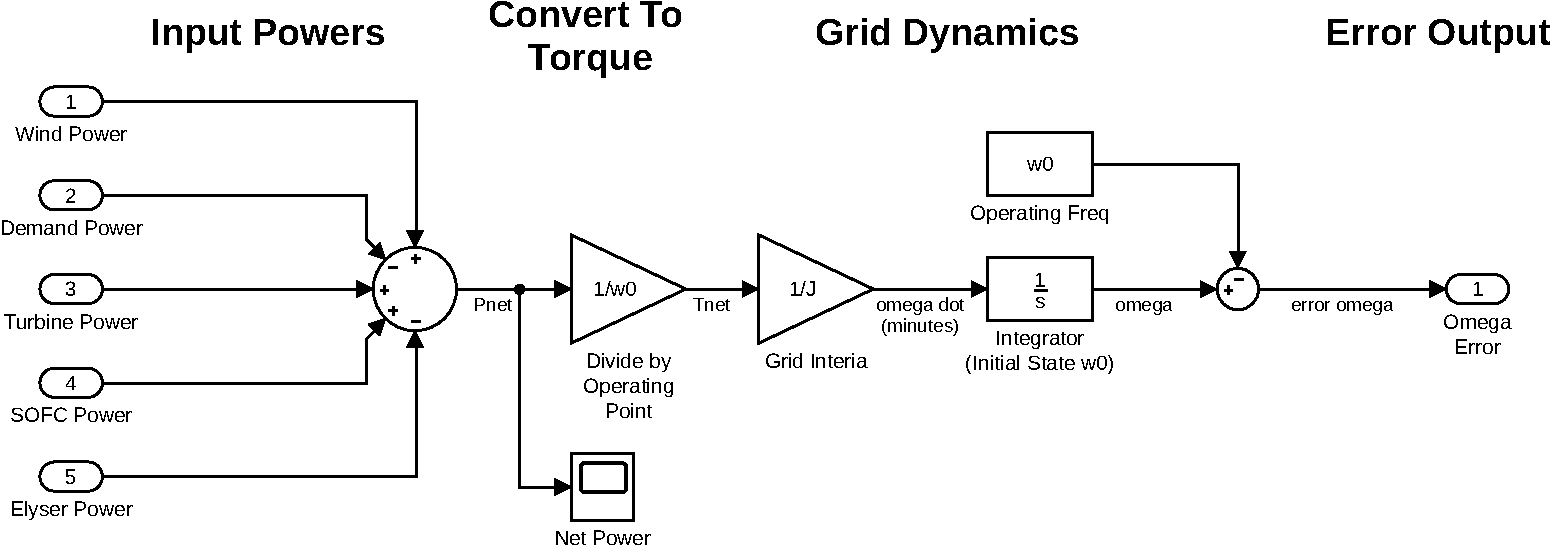
\includegraphics[scale=0.65]{images/plant2/grid.pdf}
    \caption{Grid Dynamics using Swing Equation.}
        \label{fig:grid}
\end{figure}


%\subsection{Simulation Results}

\begin{figure}
\centering
        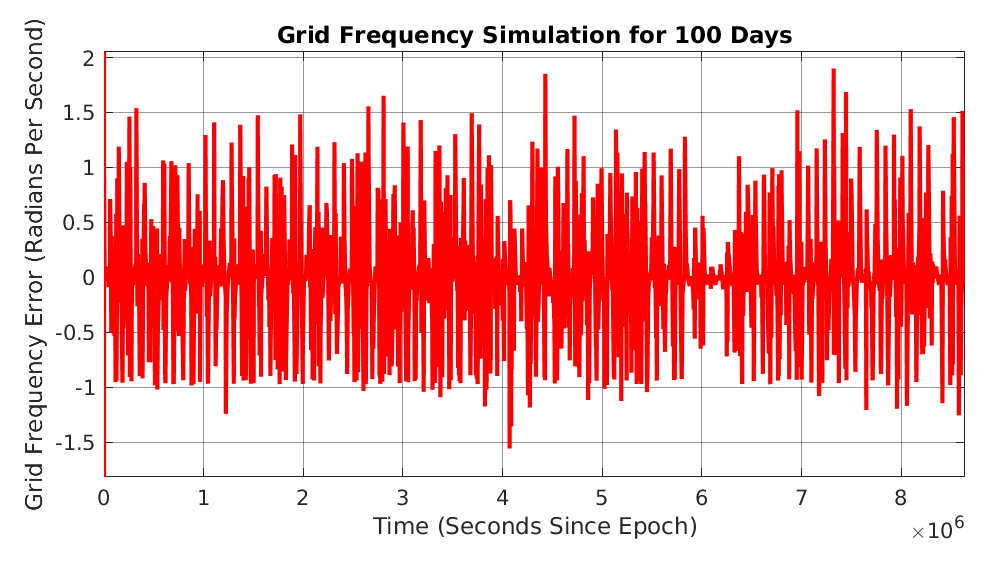
\includegraphics[scale=0.85]{images/results/omega100day.eps}
    \caption{Original specification for frequency was achieved.}
        \label{fig:grid}
\end{figure}
\begin{figure}
\centering
        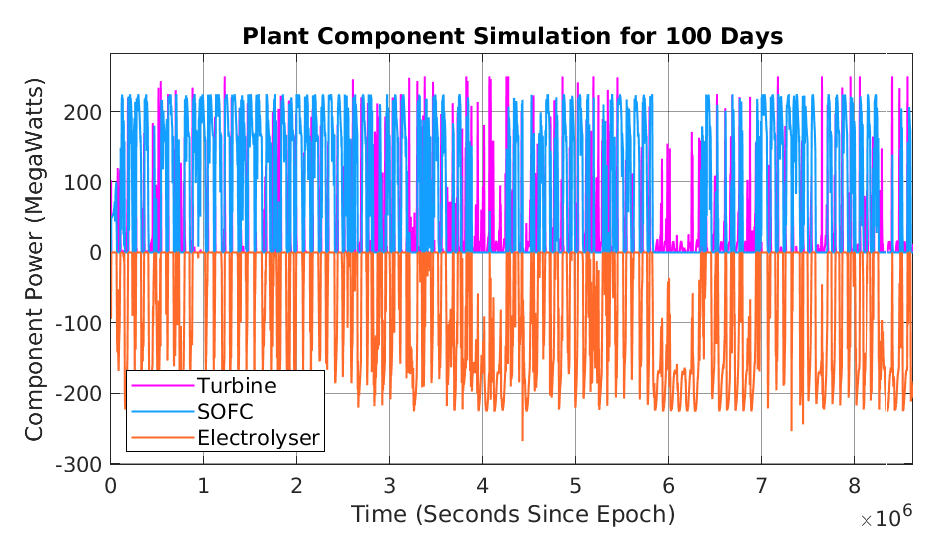
\includegraphics[scale=0.85]{images/results/comp100day.eps}
    \caption{Controller worked hard to ensure the grid was stable.}
        \label{fig:grid}
\end{figure}
\begin{figure}
\centering
        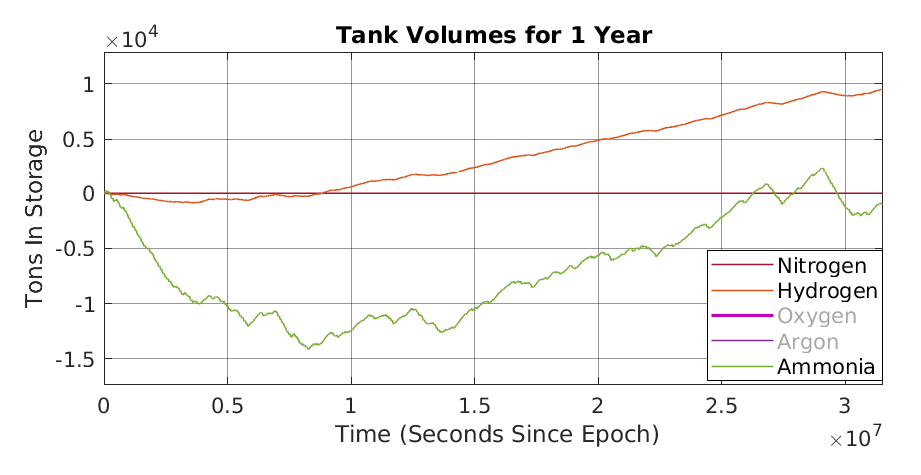
\includegraphics[scale=0.85]{images/results/tanks.eps}
    \caption{No large excess of material was produced, and viability was confirmed.}
        \label{fig:grid}
\end{figure}